\section{Allocation of time and resources}
\todo[inline]{In order for the team to get a complete overview of the time resources available for the project a Gantt diagram was created. To decide and log how the team wanted to distribute the work load between different parts of the project, a work breakdown structure was created. These are shown and explained in detail in the next two subchapters.}

\subsection{Gantt diagram}
\label{sec:gantt}

A Gantt diagram gives an overview of the overall time line of a project. The diagram orders items chronologically to easily show the projected state of the project at any given time. These items can represent milestones in the project, sprints, deadlines and team downtime. 

The Gantt diagram for the project is shown in figure~\ref{fig:gantt}. The sprints are shown as blue rectangles and represent the team's working hours. The red rectangle indicates the school trip to China in April that the whole team attended. The blue diamonds indicate milestones, or deadlines for delivery of some major part of the project.


\begin{figure}[H]
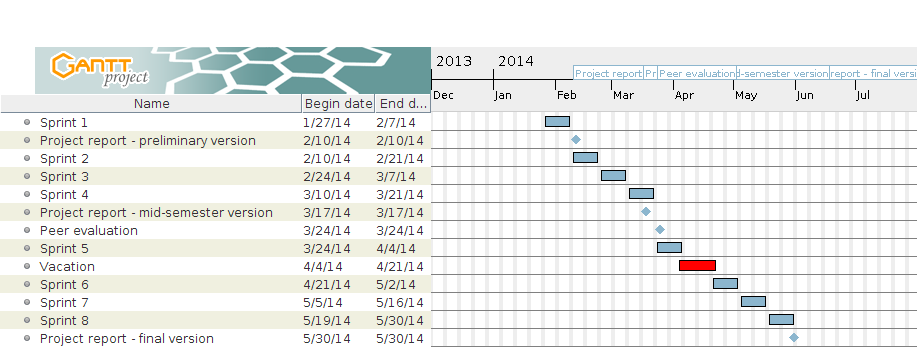
\includegraphics[width=\textwidth]{ch/projectManagement/fig/gantt.png}
\caption{The Gantt diagram with sprints and milestones.}
\label{fig:gantt}
\end{figure}
